\documentclass{beamer}
\usepackage{ucs}
\usepackage[utf8x]{inputenc}
\usepackage[T1]{fontenc}

\usepackage{graphicx}
\usepackage{tipa}

\begin{document}
\title{Pedagogiske program og språkteknologi}   
\author{Lene Antonsen \\ Senter for samisk språkteknologi, Humanistisk Fakultet\\ \begin{figure}  \scalebox{0.10}[0.10]{
\includegraphics{img/LogoSamisk}} \end{figure}} 
\date{} 


\frame{\titlepage} 

%\frame{\frametitle{Table of contents}\tableofcontents} 


%\section{Section no.1} 

\frame{\frametitle{Prosjekt: Interaktive samiskspråklige læremidler}
%\begin{block}{ }
%\textit{http://giellatekno.uit.no/oahpa/}\\
%\end{block}{ }
\begin{block}{Arbeidsgruppe:}
Lene Antonsen, Biret Ánne Bals Baal, \\ Saara Huhmarniemi, Trond Trosterud
\end{block}{ }
\begin{block}{ }
Sametinget og Universitetet i Tromsø har finansiert prosjektet
\end{block}{ }

}

\frame{\frametitle{Pedagogiske programmer}

Det er vanligvis ikke spåkteknologi i pedagogiske programmer, men
\begin{itemize}
\item multiple choice 
\item stringmatch, f.eks. \textit{jentene} = 7 bokstaver: jentene
\end{itemize} %\pause
%\begin{block}{ }
%Spåkteknologi:
%\begin{itemize}
%\item analyse, f.eks. \textit{viesus} = \textit{viessu} N Sg Loc
%\end{itemize}
%\end{block}{ }
}

\frame{\frametitle{Multiple choice}

http://www.edu.fi/oppimateriaalit/suomeaolehyva/soh1/soh1-kpl4-h3.htm
\scalebox{.45}[.45]{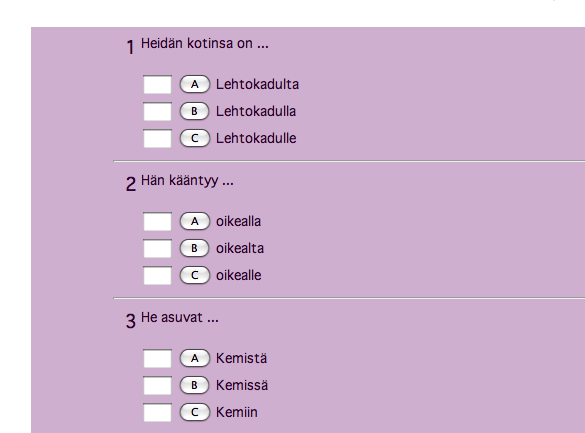
\includegraphics{img/finsk_mc-png}}
}

\frame{\frametitle{Stringmatch}

http://www.auburn.edu/forlang/russian/ \\
\scalebox{.5}[.5]{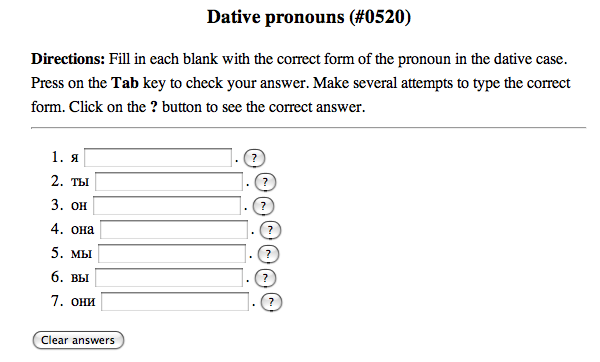
\includegraphics{img/ruossa_stringmatch.png}}

}


\frame{\frametitle{Språkteknologi: "morfologisk automat"}

\scalebox{.13}[.13]{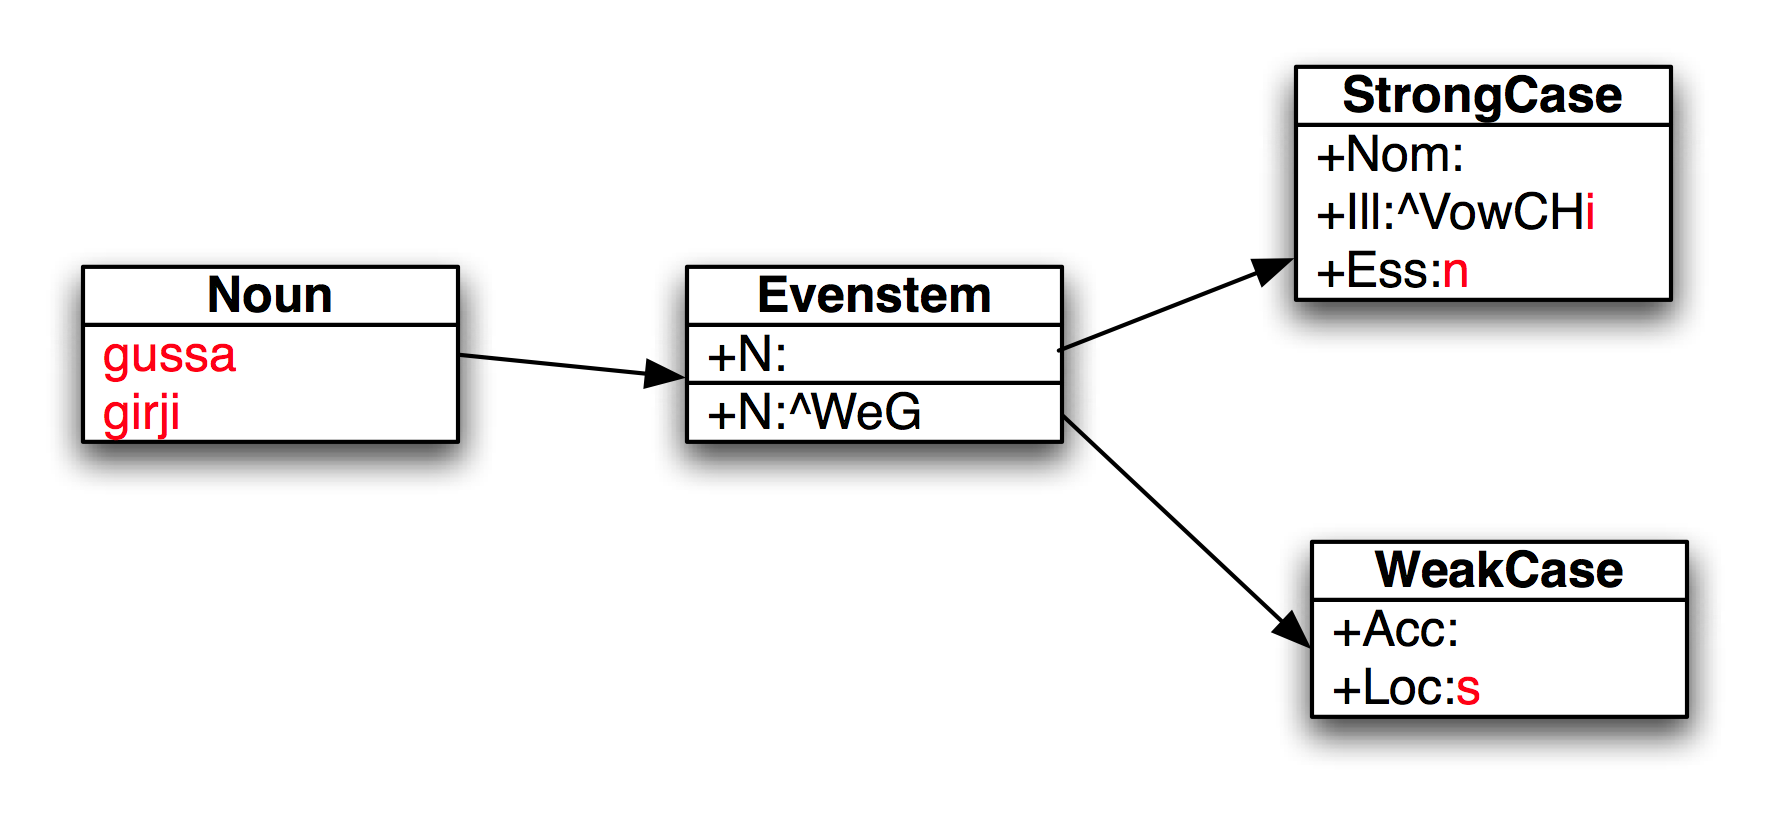
\includegraphics{img/automat.png}} \\
gussa $\rightarrow$ gussa (Nom), gussii (Ill), gussan (Ess), gusa (Acc),\\ gusas (Loc) \\
\begin{block}{ }
girji $\rightarrow$ girji (Nom), girjái (Ill), girjin (Ess), girjji (Acc), girjjis (Loc)
\end{block}{ }

}



%\frame{\frametitle{ }

%\scalebox{.19}[.19]{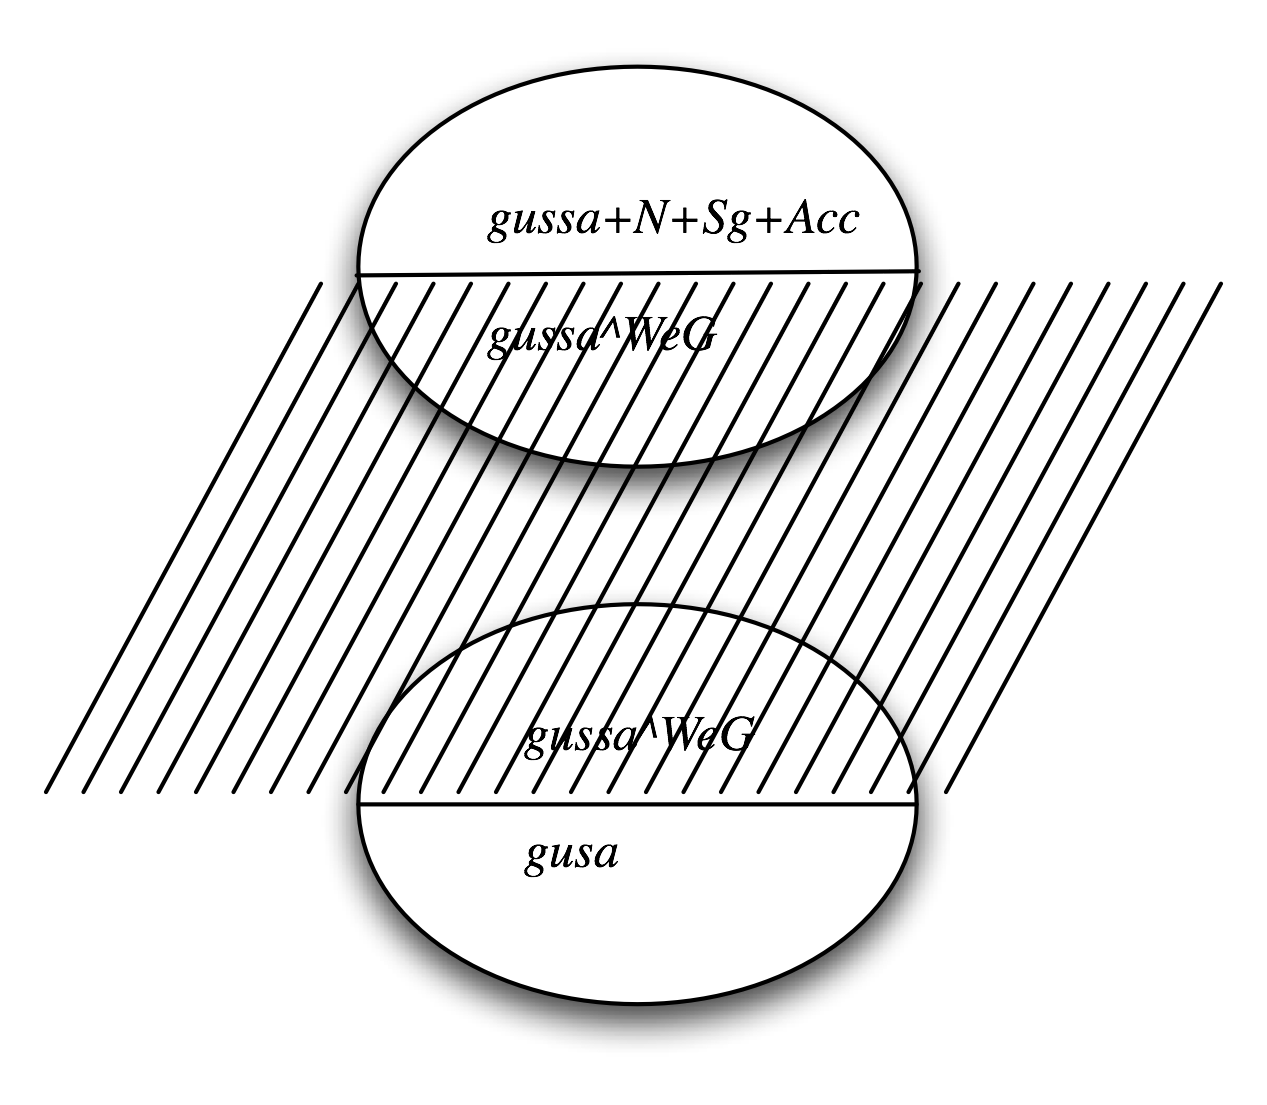
\includegraphics{img/composedautom.png}}
%}

\frame{\frametitle{http://giellatekno.uit.no}

\scalebox{.7}[.7]{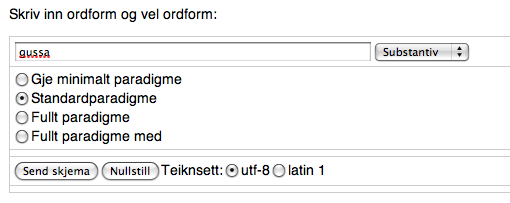
\includegraphics{img/gussaquestion.png}}
}
\frame{\frametitle{"gussa"-paradigme}

\scalebox{.55}[.55]{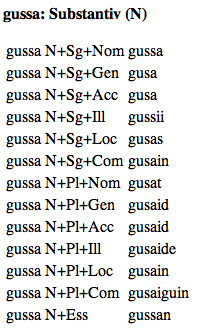
\includegraphics{img/gussa_paradigm.png}}
}


\frame{\frametitle{Homonymi}

\scalebox{.7}[.7]{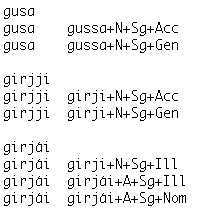
\includegraphics{img/fullautom.png}}
}

\frame{\frametitle{http://decentius.hit.uib.no/cl/cgp/test.html}

\scalebox{.6}[.6]{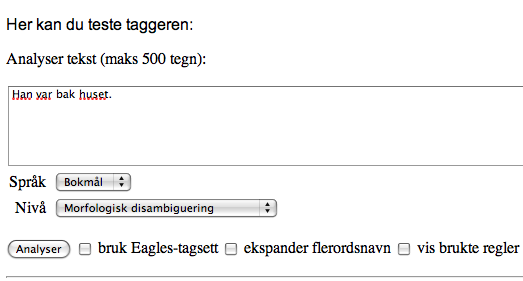
\includegraphics{img/norsk_setning.png}}
}

\frame{\frametitle{Multitagging}

\scalebox{.6}[.6]{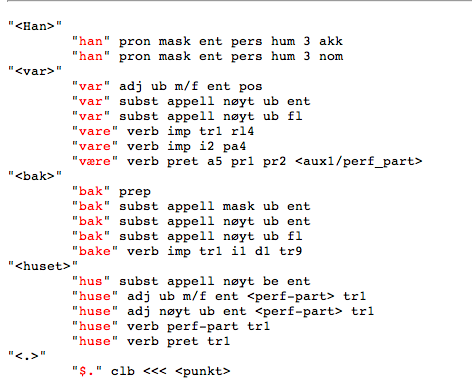
\includegraphics{img/norsk_multi.png}}
}

\frame{\frametitle{Morfologisk disambiguering}

\scalebox{.6}[.6]{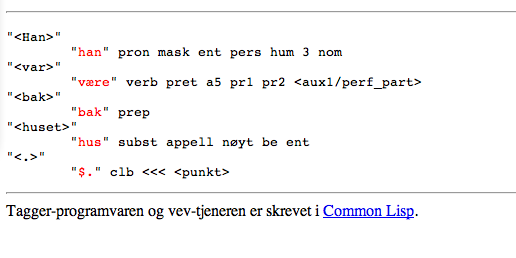
\includegraphics{img/norsk_dis.png}}
}

\frame{\frametitle{Stavekontroll}

\scalebox{.5}[.5]{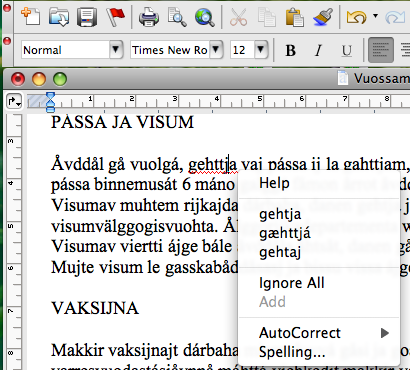
\includegraphics{img/corr-smj-text.png}}
}

\frame{\frametitle{Digital fullformsordbok}

\scalebox{.45}[.45]{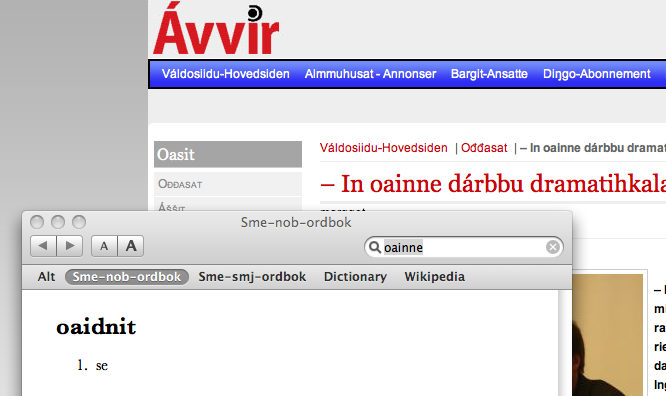
\includegraphics{img/macdic.png}}
}



\frame{\frametitle{Visual Interactive Syntax Learning - VISL}
\begin{block}{ }
\textbf{Lære grammatikk:}\\
\end{block}{ }

Mest ordklasser og syntaks, men også litt ordbøyning og quiz.\\
\begin{block}{ }
\scriptsize{arabisk,
bosnisk,
dansk,
engelsk,
esperando,
estonisk,
færøysk,
finsk,
fransk,
tysk,
gresk,
grønlansk,
islandsk,
italiensk,
japansk,
latin,
latvisk,
nederlandsk, 
nordsamisk,
norsk bokmål, 
nynorsk,
portugisisk,
rumensk,
spansk,
svensk}	 
\end{block}{ }


\begin{block}{ }
Syd-dansk Universitet har laget teknologien. \\
Vi har lagt til 1600 analyserte nordsamiske setninger.
\end{block}{ }

}

\frame{\frametitle{VISL - Paintbox}
\scalebox{2.0}[2.0]{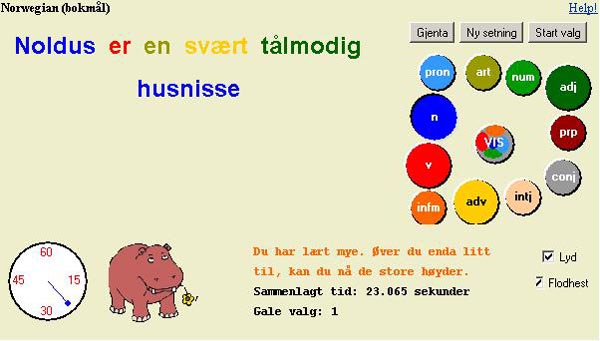
\includegraphics{img/nolduspaintklipp600.png}}
}

\frame{\frametitle{VISL - Shooting Gallery}
\scalebox{.45}[.45]{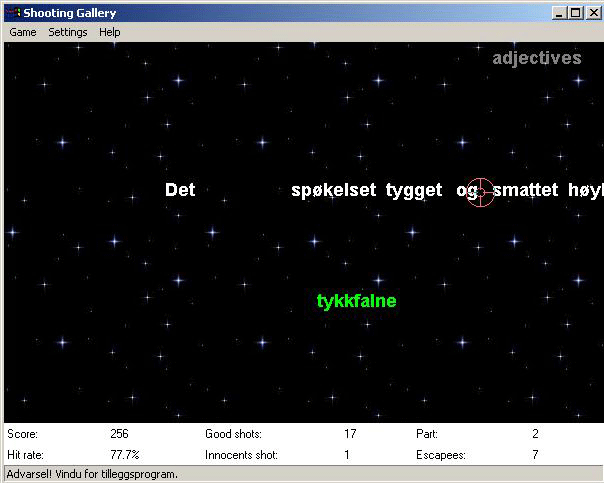
\includegraphics{img/shootingg.png}}
}

\frame{\frametitle{VISL - Syntris}
\scalebox{2.0}[2.0]{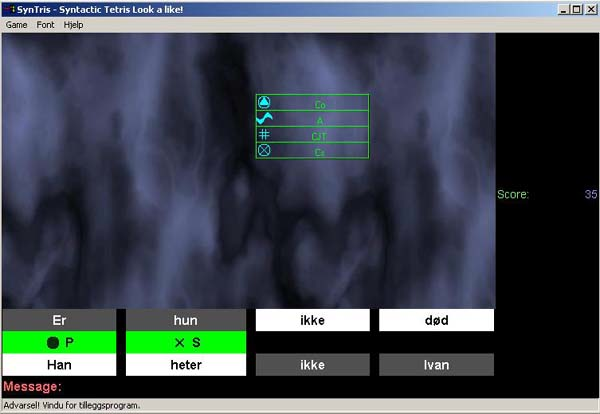
\includegraphics{img/syntris600.png}}
}
\frame{\frametitle{VISL - Wordfall}
\scalebox{.5}[.5]{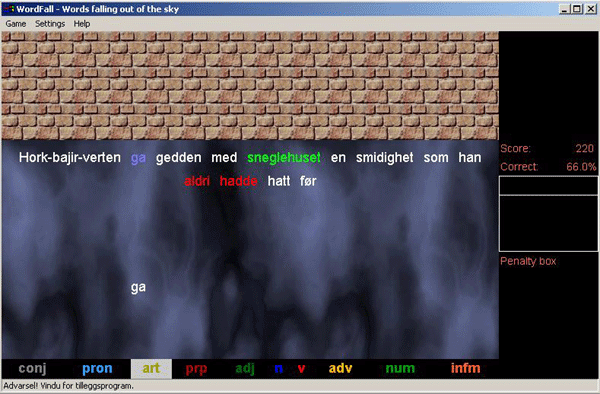
\includegraphics{img/wordfall600.png}}
}

\frame{\frametitle{VISL - Setningstre}
\scalebox{.43}[.45]{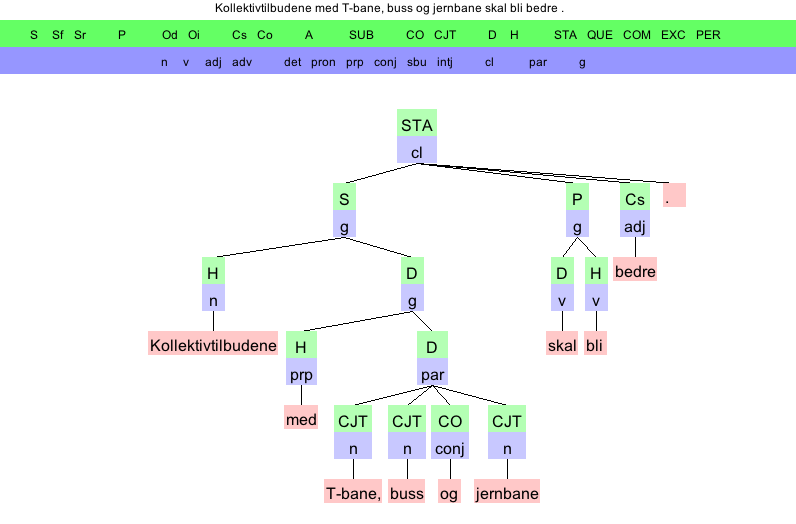
\includegraphics{img/setningstre_no.png}}
}
\frame{\frametitle{VISL - KillerFiller}
\scalebox{.55}[.55]{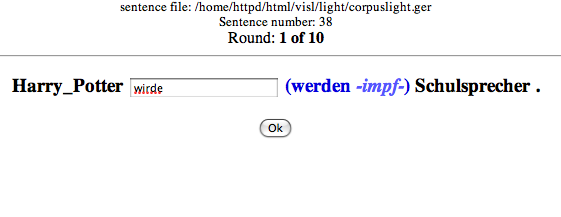
\includegraphics{img/Killer_ty_question.png}}
}
\frame{\frametitle{VISL - KillerFiller}
\scalebox{.55}[.55]{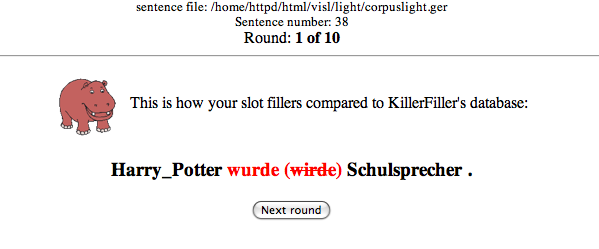
\includegraphics{img/killer_ty_answer.png}}
}

\frame{\frametitle{VISL - AnimalQuiz}
\scalebox{.45}[.45]{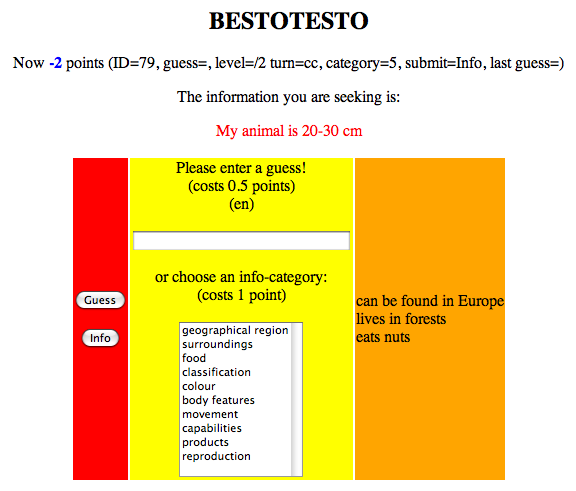
\includegraphics{img/bestotesto.png}}
}


\frame{\frametitle{http://giellatekno.uit.no/oahpa} 
\scalebox{.33}[.33]{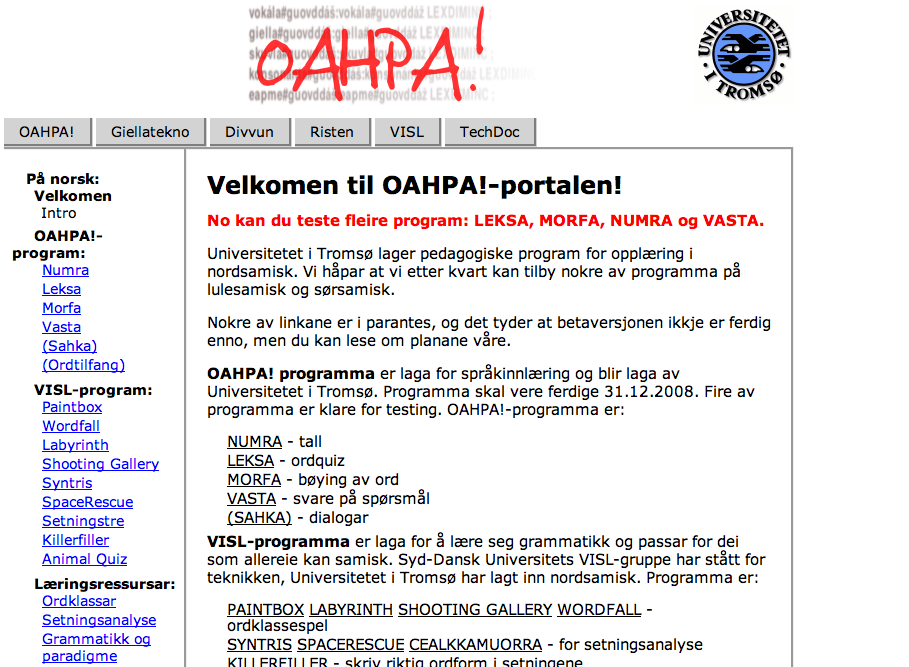
\includegraphics{img/oahpadoc.png}}
}


\frame{\frametitle{http://www.tekstlab.uio.no/grei/} 
\scalebox{.34}[.34]{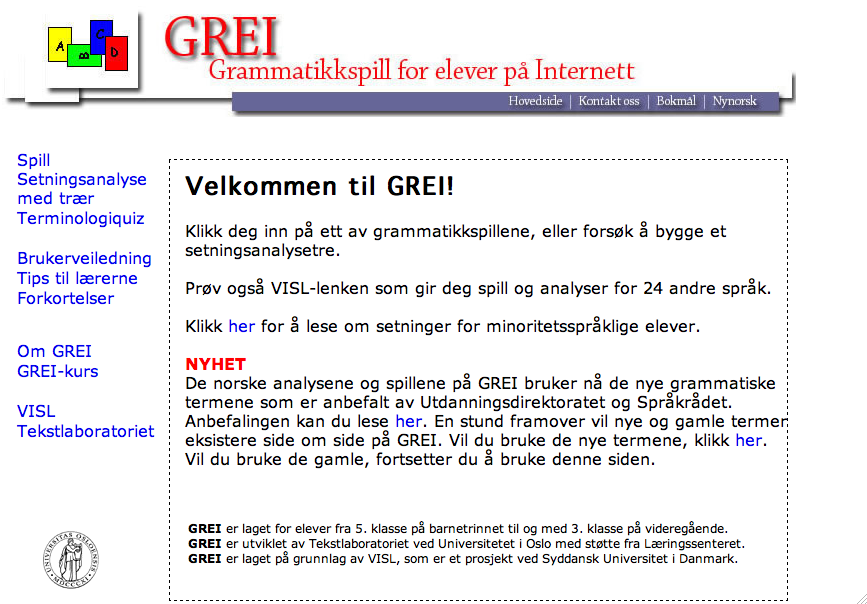
\includegraphics{img/grei.png}}
}


\frame{\frametitle{OAHPA}
\begin{block}{ }
\textbf{Programmer for dem som lærer seg nordsamisk:}\\
\end{block}{}

\begin{description}
\item [\textbf{Leksa}:] Sátnequiz - samisk/norsk og norsk/samisk
\item [\textbf{Numra}:] Trene på tall
\item [\textbf{Morfa}:] Trene på å bøye ord, også i setninger
\item [\textbf{Vasta}:] Trene på å svare på spørsmål
\item [\textbf{Sahka}:] Delta i dialog om et tema
\end{description}

\begin{block}{ }
Programmene lages ved UiT og ligger på server på internett. \\ De kan lages for andre språk også - v.hj. av analysator.
\end{block}{ }

}



\frame{\frametitle{Morfa} 
\scalebox{0.50}[0.50]{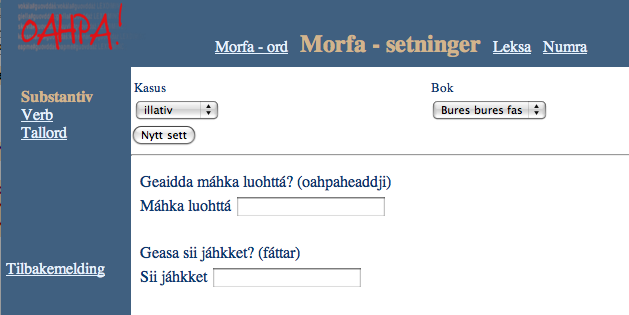
\includegraphics{img/morfa_cealkagat.png}}
}



\frame{\frametitle{Vasta -- Trene på å svare på spørsmål} 
\scalebox{0.90}[0.90]{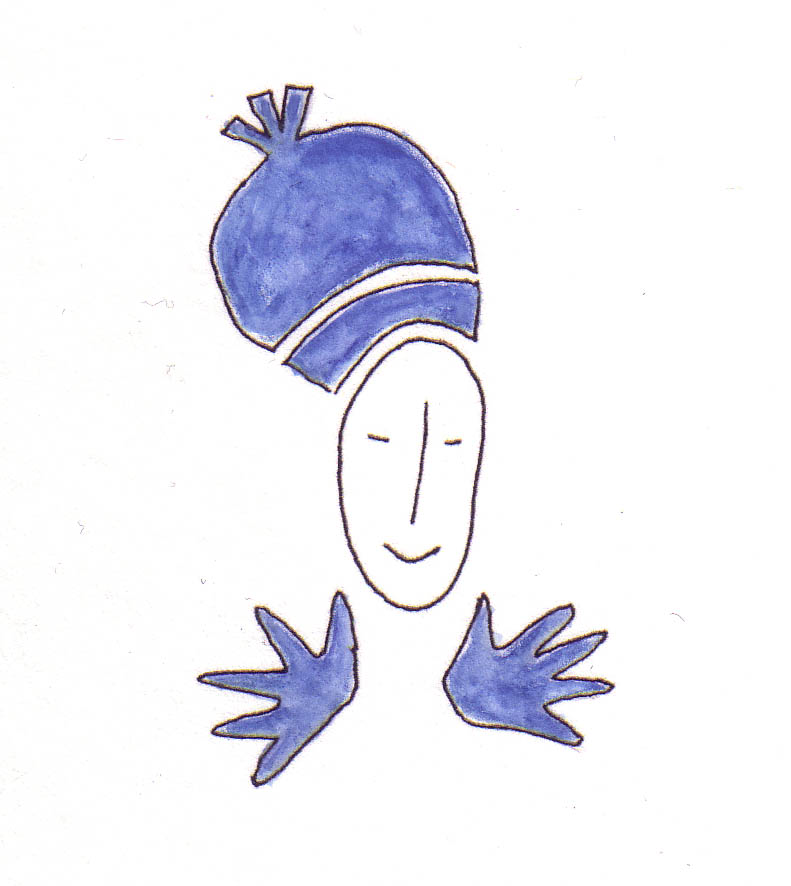
\includegraphics{img/vasta.png}} \\
}




\frame{\frametitle{Maid don lohket ikte? (Hva leste du i går?)} 

Akseptable svar:
\begin{itemize}
\item Mun han lohken ollu áviissaid. (Jeg PART leste mye aviser.) 
\item Ikte mun gal lohken buori girjji. (I går leste jeg PART ei god bok.)
\item In lohkan maidege. (Jeg leste ingenting.)
\item Ikte in lohkan. (I går leste jeg ikke.)
\end{itemize}
}

\frame{\frametitle{Maid don lohket ikte?  (Hva leste du i går?)} 

Vasta-programmet veileder på svaret ikke er akseptabelt:
\begin{itemize}
\item Mun \textbf{lohket} ollu áviissaid. \\ $\rightarrow$ Husk kongruens mellom subjekt og verbal.  
\item Mun lohken ollu \textbf{áviissat}. \\ $\rightarrow$ Objektet skal være i akkusativ. 
\item \textbf{Don lohket} ollu áviissaid. \\ $\rightarrow$ Er du sikker på at du svarer i riktig person?  
\end{itemize}
}

\frame{\frametitle{Vasta} 
\scalebox{0.5}[0.5]{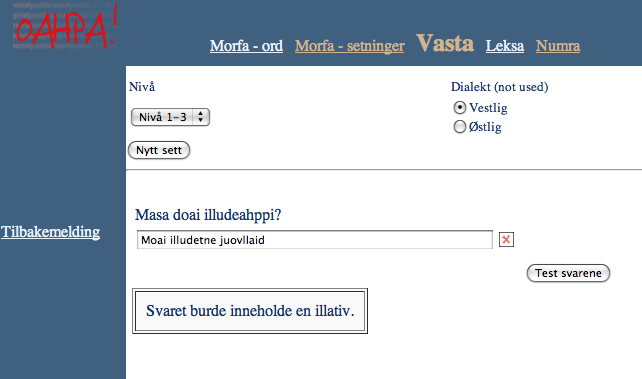
\includegraphics{img/vasta2.png}}
}


\frame{\frametitle{Vår visjon} 
Programmet skal veilede brukeren på samme måte som en lærer gjør.
}


%\subsection{Lists II}
%\frame{\frametitle{numbered lists}
%\begin{enumerate}
%\item Introduction to  \LaTeX  
%\item Course 2 
%\item Termpapers and presentations with \LaTeX 
%\item Beamer class
%\end{enumerate}
%}
%\frame{\frametitle{numbered lists with pause}
%\begin{enumerate}
%\item Introduction to  \LaTeX \pause 
%\item Course 2 \pause 
%\item Termpapers and presentations with \LaTeX \pause 
%\item Beamer class
%\end{enumerate}
%}
%
%\section{Section no.3} 
%\subsection{Tables}
%\frame{\frametitle{Tables}
%\begin{tabular}{|c|c|c|}
%\hline
%\textbf{Date} & \textbf{Instructor} & \textbf{Title} \\
%\hline
%WS 04/05 & Sascha Frank & First steps with  \LaTeX  \\
%\hline
%SS 05 & Sascha Frank & \LaTeX \ Course serial \\
%\hline
%\end{tabular}}
%
%
%\frame{\frametitle{Tables with pause}
%\begin{tabular}{c c c}
%A & B & C \\ 
%\pause 
%1 & 2 & 3 \\  
%\pause 
%A & B & C \\ 
%\end{tabular} }
%
%
%\section{Section no. 4}
%\subsection{blocs}
%\frame{\frametitle{blocs}
%
%\begin{block}{title of the bloc}
%bloc text
%\end{block}
%
%\begin{exampleblock}{title of the bloc}
%bloc text
%\end{exampleblock}
%
%
%\begin{alertblock}{title of the bloc}
%bloc text
%\end{alertblock}
\end{document}

